% CENG467 Final Project Presentation
% CodeEnhancer Model Comparison — 10-minute presentation
\documentclass[aspectratio=169]{beamer}

\usetheme{Madrid}
\usecolortheme{whale}
\setbeamertemplate{blocks}[rounded][shadow=false]
\setbeamertemplate{navigation symbols}{}
\setbeamertemplate{footline}[frame number]

\usepackage[utf8]{inputenc}
\usepackage[T1]{fontenc}
\usepackage{graphicx}
\usepackage{booktabs}
\usepackage{multirow}
\usepackage{xcolor}
\usepackage{tikz}

% ─── Color customization ───
\definecolor{iyte_blue}{RGB}{0, 56, 116}
\definecolor{iyte_light}{RGB}{173, 216, 230}
\setbeamercolor{frametitle}{bg=iyte_blue, fg=white}
\setbeamercolor{title}{fg=white}
\setbeamercolor{structure}{fg=iyte_blue}
\setbeamercolor{block title}{bg=iyte_blue, fg=white}

% ─── Title info ───
\title[CodeEnhancer Model Comparison]{\textbf{CodeEnhancer Model Comparison}}
\subtitle{Evaluating Open-Source LLMs for Secure Code Generation \\ \vspace{0.3em} \small Term Project Final Presentation}
\author{Ali Ekin Özçetin \and Ali Sezer Uysal \and Mert Güner}
\institute{Izmir Institute of Technology \\ \small Advisor: Prof.\ Dr.\ Aytu\u{g} Onan}
\date{CENG467 --- June 2026}

\begin{document}

% ─────────────────────────────────────────────
% SLIDE 1 — Title
% ─────────────────────────────────────────────
\begin{frame}
  \titlepage
\end{frame}

% ─────────────────────────────────────────────
% SLIDE 2 — Motivation
% ─────────────────────────────────────────────
\begin{frame}{The Problem}
  \begin{columns}[T]
    \begin{column}{0.55\textwidth}
      \begin{block}{LLMs Write Vulnerable Code}
        \begin{itemize}
          \item GitHub Copilot: \textbf{$\sim$40\%} of generated programs contain vulnerabilities
          \item Common weaknesses: SQL injection, command injection, path traversal
          \item Developers using AI assistants write \textbf{less secure code}
        \end{itemize}
      \end{block}
      \vspace{0.4em}
      \begin{alertblock}{Additional Challenge}
        When asked to review their own code, LLMs often \textbf{miss the same mistakes} they just made --- they need an external checker to catch errors reliably
      \end{alertblock}
    \end{column}
    \begin{column}{0.42\textwidth}
      \centering
      \vspace{1em}
      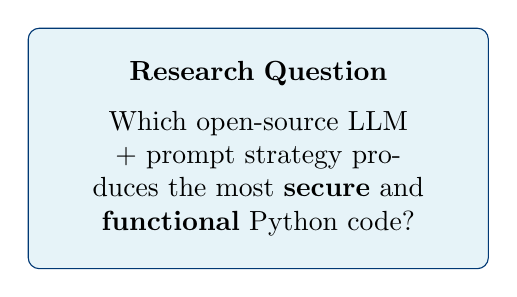
\begin{tikzpicture}
        \node[draw=iyte_blue, rounded corners, fill=iyte_light!30,
              text width=5cm, align=center, inner sep=12pt] {
          \textbf{Research Question} \\[0.6em]
          Which open-source LLM + prompt strategy produces the most
          \textbf{secure} and \textbf{functional} Python code?
        };
      \end{tikzpicture}
    \end{column}
  \end{columns}
\end{frame}

% ─────────────────────────────────────────────
% SLIDE 3 — Our Approach
% ─────────────────────────────────────────────
\begin{frame}{Our Approach: Extending CodeEnhancer}
  \begin{columns}[T]
    \begin{column}{0.48\textwidth}
      \begin{block}{Original Framework}
        \begin{itemize}
          \item GPT-4o only — closed source
          \item Same model generates \emph{and} judges
          \item 82.8\% vulnerability resolution
        \end{itemize}
      \end{block}
      \vspace{0.4em}
      \begin{block}{Our Contributions}
        \begin{itemize}
          \item \textbf{5 open-source LLMs} via Ollama
          \item \textbf{3 prompt strategies} compared
          \item \textbf{GPT-4o-mini} as independent judge
          \item 1,215 total scenarios
          \item Zero cost for local generation
        \end{itemize}
      \end{block}
    \end{column}
    \begin{column}{0.48\textwidth}
      \centering
      \vspace{0.3em}
      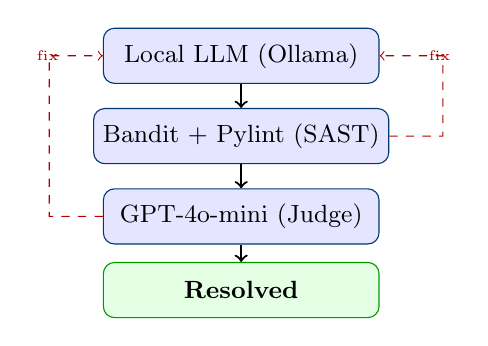
\begin{tikzpicture}[scale=0.85, every node/.style={font=\small}]
        \node[draw=iyte_blue, fill=blue!10, rounded corners,
              minimum width=3.5cm, minimum height=0.7cm, align=center]
              (gen) at (0,3.5) {Local LLM (Ollama)};
        \node[draw=iyte_blue, fill=blue!10, rounded corners,
              minimum width=3.5cm, minimum height=0.7cm, align=center]
              (sast) at (0,2.3) {Bandit + Pylint (SAST)};
        \node[draw=iyte_blue, fill=blue!10, rounded corners,
              minimum width=3.5cm, minimum height=0.7cm, align=center]
              (judge) at (0,1.1) {GPT-4o-mini (Judge)};
        \node[draw=green!60!black, fill=green!10, rounded corners,
              minimum width=3.5cm, minimum height=0.7cm, align=center]
              (done) at (0,0) {\textbf{Resolved}};
        \draw[->, thick] (gen) -- (sast);
        \draw[->, thick] (sast) -- (judge);
        \draw[->, thick] (judge) -- (done);
        \draw[->, dashed, red!70!black]
          (sast.east) -- ++(0.8,0) -- ++(0,1.2) -- (gen.east)
          node[midway, right, xshift=0.1cm]{\tiny fix};
        \draw[->, dashed, red!70!black]
          (judge.west) -- ++(-0.8,0) -- ++(0,2.4) -- (gen.west)
          node[midway, left, xshift=-0.1cm]{\tiny fix};
      \end{tikzpicture}
      \vspace{0.5em}

      \small Up to \textbf{5} repair iterations per scenario
    \end{column}
  \end{columns}
\end{frame}

% ─────────────────────────────────────────────
% SLIDE 4 — Experiment Setup
% ─────────────────────────────────────────────
\begin{frame}{Experiment Setup}
  \begin{columns}[T]
    \begin{column}{0.48\textwidth}
      \begin{block}{5 Models Tested}
        \begin{tabular}{ll}
          \toprule
          \textbf{Model} & \textbf{Type} \\
          \midrule
          Qwen 2.5 Coder 7B   & Code-spec. \\
          DeepSeek-Coder 6.7B & Code-spec. \\
          Llama 3.1 8B        & General \\
          Gemma 2 9B          & General \\
          Mistral 7B          & General \\
          \bottomrule
        \end{tabular}
      \end{block}
    \end{column}
    \begin{column}{0.48\textwidth}
      \begin{block}{3 Prompt Strategies}
        \begin{itemize}
          \item \textbf{Zero-shot:} Task only, no examples
          \item \textbf{Few-shot:} 5 secure code examples\\(CWE-78, 89, 502, 434, 22)
          \item \textbf{Chain-of-Thought:} 4-step security reasoning
        \end{itemize}
      \end{block}
      \vspace{0.3em}
      \begin{block}{Dataset}
        \textbf{LLMSecEval:} 81 Python prompts, 12 CWE categories \\[0.3em]
        \textbf{Total:} $5 \times 3 \times 81 =$ \textbf{1,215 scenarios}
      \end{block}
    \end{column}
  \end{columns}
\end{frame}

% ─────────────────────────────────────────────
% SLIDE 5 — Resolution Rates (main result)
% ─────────────────────────────────────────────
\begin{frame}{Result 1: Final Resolution Rates}
  \centering
  \includegraphics[width=0.72\textwidth]{figures/fig2_resolution_rate.png}
  \vspace{0.3em}

  \begin{columns}[T]
    \begin{column}{0.48\textwidth}
      \small \textbf{Qwen 2.5 Coder 7B} achieved the highest average resolution rate at \textbf{80.2\%}, followed by DeepSeek-Coder (77.3\%) and Llama 3.1 (75.7\%). Models trained specifically on code data clearly outperform general-purpose models.
    \end{column}
    \begin{column}{0.48\textwidth}
      \small \textbf{Mistral 7B} performed the worst at \textbf{56.0\%}, struggling to fix code even after multiple repair attempts. \textbf{Gemma 2 9B} also fell short at 63.8\%, despite having the most parameters among the tested models.
    \end{column}
  \end{columns}
\end{frame}

% ─────────────────────────────────────────────
% SLIDE 6 — Code vs General + Judge Analysis
% ─────────────────────────────────────────────
\begin{frame}{Result 2: Code-Specialized vs.\ General-Purpose}
  \begin{columns}[T]
    \begin{column}{0.60\textwidth}
      \centering
      \includegraphics[width=\textwidth]{figures/fig8_code_vs_general.png}
    \end{column}
    \begin{column}{0.37\textwidth}
      \vspace{1em}
      Models trained specifically on code data (\textbf{Qwen}, \textbf{DeepSeek}) achieved higher resolution rates and needed fewer repair attempts.
      \vspace{0.8em}

      General-purpose models (\textbf{Gemma}, \textbf{Mistral}) struggled more with both security fixes and functional correctness.
    \end{column}
  \end{columns}
\end{frame}

% ─────────────────────────────────────────────
% SLIDE 7 — Self-Assessment Bias
% ─────────────────────────────────────────────
\begin{frame}{Result 3: Decoupling the Judge Matters}
  \begin{columns}[T]
    \begin{column}{0.52\textwidth}
      \centering
      \includegraphics[width=\textwidth]{figures/fig10_judge_analysis.png}
    \end{column}
    \begin{column}{0.45\textwidth}
      \vspace{0.5em}
      \textbf{The Problem:} When a model checks its own code, it tends to approve the same mistakes it just made.
      \vspace{0.8em}

      \begin{tabular}{lrr}
        \toprule
        \textbf{Model} & \textbf{Self} & \textbf{Ext.} \\
        \midrule
        Llama 3.1 & 0\% & \textbf{75.7\%} \\
        \bottomrule
      \end{tabular}
      \vspace{0.8em}

      \textbf{The Fix:} We used \textbf{GPT-4o-mini} as a separate, independent checker. It evaluates code without any bias toward the model that wrote it.
      \vspace{0.5em}

      \textbf{Mistral 7B} received the most failed checks --- it kept generating incomplete code even after passing the security scan.
    \end{column}
  \end{columns}
\end{frame}

% ─────────────────────────────────────────────
% SLIDE 8 — Prompt Strategy + CWE Heatmap
% ─────────────────────────────────────────────
\begin{frame}{Result 4: Prompt Strategy and CWE Analysis}
  \begin{columns}[T]
    \begin{column}{0.50\textwidth}
      \centering
      \includegraphics[width=\textwidth]{figures/fig4_cwe_heatmap.png}
      \vspace{0.3em}

      \small \textbf{CWE-78} (command injection) and \textbf{CWE-502} (deserialization) were the hardest categories --- no model could fully eliminate them.
    \end{column}
    \begin{column}{0.47\textwidth}
      \vspace{0.3em}
      \begin{tabular}{lrr}
        \toprule
        \textbf{Strategy} & \textbf{Res.} & \textbf{Iter.} \\
        \midrule
        Few-shot  & \textbf{73.3\%} & \textbf{2.66} \\
        Zero-shot & 71.8\%          & 2.72 \\
        CoT       & 66.7\%          & 2.87 \\
        \bottomrule
      \end{tabular}
      \vspace{0.6em}

      \textbf{Few-shot} works best --- showing secure code examples before the task guides the model effectively.
      \vspace{0.5em}

      \textbf{Chain-of-Thought} scored the lowest. The long reasoning text consumed the model's context, leaving less room for repair instructions.
    \end{column}
  \end{columns}
\end{frame}

% ─────────────────────────────────────────────
% SLIDE 9 — Few-Shot Generalization
% ─────────────────────────────────────────────
\begin{frame}{Result 5: Few-Shot Generalizes to Unseen CWEs}
  \centering
  \includegraphics[width=0.62\textwidth]{figures/fig9_seen_unseen_cwe.png}
  \vspace{0.3em}

  \begin{columns}[T]
    \begin{column}{0.48\textwidth}
      \small Our examples covered only 5 specific CWE types. Yet models scored \textbf{higher on vulnerability types they had never seen} --- Qwen reached 84.4\% on unseen vs.\ 80.6\% on seen CWEs.
    \end{column}
    \begin{column}{0.48\textwidth}
      \small Models did not just memorize the examples. They learned a \textbf{general rule} --- check inputs, use safe functions, avoid dangerous calls --- and applied it to new situations.
    \end{column}
  \end{columns}
\end{frame}

% ─────────────────────────────────────────────
% SLIDE 10 — Key Findings
% ─────────────────────────────────────────────
\begin{frame}{Key Findings}
  \begin{columns}[T]
    \begin{column}{0.50\textwidth}
      \begin{block}{Best Model}
        \textbf{Qwen 2.5 Coder 7B} --- 80.2\% resolution \\
        Code-specialized $>$ general-purpose
      \end{block}
      \vspace{0.35em}
      \begin{block}{Best Strategy}
        \textbf{Few-shot} --- 73.3\% res., 2.66 avg.\ iterations
      \end{block}
      \vspace{0.35em}
      \begin{block}{Decouple the Judge}
        Essential: Llama went \textbf{0\%} $\rightarrow$ \textbf{75.7\%}
      \end{block}
    \end{column}
    \begin{column}{0.47\textwidth}
      \begin{block}{CoT Paradox}
        Fewer initial bugs but worse repair in small models
      \end{block}
      \vspace{0.35em}
      \begin{block}{Few-Shot Generalizes}
        Unseen CWEs perform equal or better than seen
      \end{block}
      \vspace{0.35em}
      \begin{alertblock}{Recommendation}
        \textbf{Qwen + Few-shot + External Judge} is the best local, cost-free secure code pipeline
      \end{alertblock}
    \end{column}
  \end{columns}
\end{frame}

% ─────────────────────────────────────────────
% SLIDE 11 — Thank you / Q&A
% ─────────────────────────────────────────────
\begin{frame}{Thank You}
  \centering
  \vspace{0.8em}
  {\Large \textbf{CodeEnhancer Model Comparison}}\\[0.4em]
  {\normalsize Evaluating Open-Source LLMs for Secure Code Generation}

  \vspace{1.2em}

  \begin{columns}[c]
    \begin{column}{0.45\textwidth}
      \centering
      \begin{block}{Team}
        Ali Ekin Özçetin \\
        Ali Sezer Uysal \\
        Mert Güner
      \end{block}
    \end{column}
    \begin{column}{0.45\textwidth}
      \centering
      \begin{block}{Repository}
        \small \url{https://github.com/Aliekinozcetin/CodeEnhancer/tree/main}
      \end{block}
    \end{column}
  \end{columns}

  \vspace{1.2em}
  {\LARGE \textbf{Questions?}}

  \vspace{0.5em}
  \tiny
  \begin{thebibliography}{9}
    \bibitem{lee2026} Lee et al., \textit{Knowledge-Based Systems} (2026)
    \bibitem{pearce2022} Pearce et al., IEEE SP (2022)
    \bibitem{olausson2024} Olausson et al., ICLR (2024)
    \bibitem{tony2023} Tony et al., MSR (2023)
  \end{thebibliography}
\end{frame}

\end{document}
